% ============================================================
%  GSP colloquium talk -- Nikola Mamic
%  20 min talk + 5 min discussion, 33/33/33 rule
%  Compiler: pdfLaTeX. FZJ theme installed globally in texmf
%  (provides beamertheme*Juelich.sty, fzj logo, placeholder image)
% ============================================================
\documentclass[aspectratio=169]{beamer}
\usetheme{Juelich}

\usepackage[T1]{fontenc}   % proper glyphs/hyphenation for accented names

% - theme settings --------------
% title page: default "image" variant (picture on top, blue band below);
% the picture comes from \titlegraphic further down.
% Section pages use the same image variant, so they look like the title slide.
\fzjset{section page=image}
% the theme's image section page prints the section name in the small subtitle font
% (it expects a \part); show it in the title font instead, talk title underneath
\makeatletter
\expandafter\let\csname beamer@@tmpop@section page@image\endcsname\relax
\makeatother
\defbeamertemplate{section page}{image}{%
  \vskip\myheadlineb%
  \leftskip 0.05\paperheight%
  \advance\rightskip 0.05\paperheight%
  \usebeamercolor[fg]{title}\usebeamerfont*{title}\strut{}\insertsection\par%
  \usebeamercolor[fg]{subtitle}\usebeamerfont{subtitle}\strut{}\inserttitle\par%
}
% long announcement title as subtitle -> use the small (9pt) subtitle font
\setbeamerfont*{subtitle}{parent=subtitle long}
% optional: "Slide 5 | 17" instead of "Slide 5" (needs two compile runs)
% \setbeamertemplate{frame number}[full]

\graphicspath{{figures/}}

% - TikZ styles ---------------
% colour code: fzjblue = simulation side, fzjorange = ML side, fzjred = problems/bugs only
% grey shades: the theme defines these only under an option, values copied from it
\providecolor{fzjgray80}{RGB}{81,81,81}
\providecolor{fzjgray50}{RGB}{156,156,156}
\usetikzlibrary{arrows.meta, positioning, calc, decorations.pathreplacing, fit, backgrounds}
\tikzset{
  box/.style      = {rounded corners=3pt, align=center, font=\footnotesize, inner sep=4pt},
  sim/.style      = {box, fill=fzjblue, text=white},
  simlight/.style = {box, fill=fzjblue!10, draw=fzjblue, text=fzjblue},
  ml/.style       = {box, fill=fzjorange},
  mllight/.style  = {box, fill=fzjorange!20, draw=fzjorange!80!black},
  bug/.style      = {box, fill=fzjred!12, draw=fzjred, text=fzjred!80!black},
  neutral/.style  = {box, fill=fzjgray, text=fzjgray80},
  arr/.style      = {-{Stealth[length=2.2mm]}, thick},
  brace/.style    = {decorate, decoration={brace, amplitude=4pt}, thick},
}

% - helpers -----------------
% figure placeholder: \figph{width}{height}{what}{how to make it}
\newcommand{\figph}[4]{%
  \tikz\node[draw=fzjblue, dashed, thick, fill=fzjblue!5, rounded corners=3pt,
    minimum width=#1, minimum height=#2, text width=#1-1.2em, align=center,
    font=\scriptsize, text=fzjblue]{\textbf{FIGURE: #3}\\[2pt]#4};}
% figure if figures/<basename>.pdf or .png exists, otherwise a placeholder naming the file:
% \figorph{basename}{width}{height}{what}{how to make it}
\newcommand{\figorph}[5]{%
  \IfFileExists{figures/#1.pdf}{\includegraphics[width=#2, height=#3, keepaspectratio]{#1.pdf}}{%
  \IfFileExists{figures/#1.png}{\includegraphics[width=#2, height=#3, keepaspectratio]{#1.png}}{%
  \figph{#2}{#3}{#4}{#5\\[2pt]\texttt{figures/\detokenize{#1}.pdf|png}}}}}
% source / credit line in the bottom-left corner, above the footer
\newcommand{\src}[1]{%
  \begin{tikzpicture}[remember picture, overlay]
    \node[anchor=south west, font=\tiny, text=fzjgray80, inner sep=0pt]
      at ([xshift=0.45cm, yshift=0.75cm]current page.south west) {#1};
  \end{tikzpicture}}
% content that only appears once a real figure exists: \iffig{basename}{with}{without}
\newcommand{\iffig}[3]{\IfFileExists{figures/#1.pdf}{#2}{\IfFileExists{figures/#1.png}{#2}{#3}}}
\newcommand{\hl}[1]{{\color{fzjblue}\textbf{#1}}}
\newsavebox{\diagbox}  % holds a diagram that is placed at one of two sizes

% - title data ----------------
\title{Towards a Foundational Model for Particle-Based Methods}
\subtitle{Scaling neural operators for large-scale plasma simulations and coupling to production codes}
\author{Nikola Mami\'c}
\institute{JSC}
\date{October 2026}   % TODO: exact colloquium date
% tiled FZJ placeholder image shipped with the theme (same as tutorial/minimal.tex);
% can later be replaced by a figure of your own
\titlegraphic{\includegraphics[width=\paperwidth]{placeholder}}

% GO20 references below: "slide N" = number printed on Sriram's slide
% (refs/go20_pif.pdf), "PDF p." = page in that file (= N + 1).
% GO20 figures only with Sriram's permission, credited "Muralikrishnan, Go20 2026".
% Figures in figures/*.pdf are made by figures/make_figures.py from SYNTHETIC
% particles -- they are illustrations, not results.

\begin{document}

% Title slide: must be OUTSIDE a frame (theme builds its own frame)
\maketitle

% ============================================================
\section{Introduction}   % third 1: everyone understands, frames 1--6
\makesection
% ============================================================

% - frame 1 - GO20: slide 3 (PDF p.4), loop redrawn
\begin{frame}{Particle--field systems and the PIC loop}
  \begin{columns}[c]
    \begin{column}{0.42\textwidth}
      \begin{itemize}
        \item \hl{Particles} move by ODEs,\\ \hl{fields} obey PDEs
        \item Coupled in both directions:\\ particles make the field,\\ the field pushes the particles
        \item Plasmas (particle-in-cell, PIC), vortex flows, \ldots
        \item Electrostatic plasma:\\ $-\nabla^2\phi = \rho/\epsilon_0,\quad E=-\nabla\phi$
      \end{itemize}
    \end{column}
    \begin{column}{0.56\textwidth}
      \centering
      \begin{tikzpicture}[every node/.style={minimum width=2.9cm, minimum height=1.0cm}]
        \node[sim] (sc) at (0, 1.55)  {\textbf{Scatter}\\[-1pt]\scriptsize charge $\to$ mesh};
        \node[sim] (so) at (2.6, 0)   {\textbf{Solve on mesh}\\[-1pt]\scriptsize $-\nabla^2\phi=\rho/\epsilon_0$};
        \node[sim] (ga) at (0, -1.55) {\textbf{Gather}\\[-1pt]\scriptsize $E$ mesh $\to$ particles};
        \node[sim] (pu) at (-2.6, 0)  {\textbf{Push}\\[-1pt]\scriptsize $\dot x=v,\ \dot v=\tfrac{q}{m}E$};
        \draw[arr, fzjblue] (sc.east) to[out=0, in=90]   (so.north);
        \draw[arr, fzjblue] (so.south) to[out=-90, in=0] (ga.east);
        \draw[arr, fzjblue] (ga.west) to[out=180, in=-90] (pu.south);
        \draw[arr, fzjblue] (pu.north) to[out=90, in=180] (sc.west);
        \node[simlight, minimum width=1.6cm, minimum height=0.6cm] (in) at (-2.9, 1.75)
          {\scriptsize Init $x, v, q$};
        \draw[arr, fzjblue] (in.east) -- ++(0.35,0) |- ([yshift=2mm]sc.west);
        \node[text=fzjgray80, font=\scriptsize] at (0,0) {one time step};
      \end{tikzpicture}
    \end{column}
  \end{columns}
\end{frame}

% - frame 2 - own illustration
\begin{frame}{From grids to Fourier modes}
  \centering
  \vspace*{4pt}
  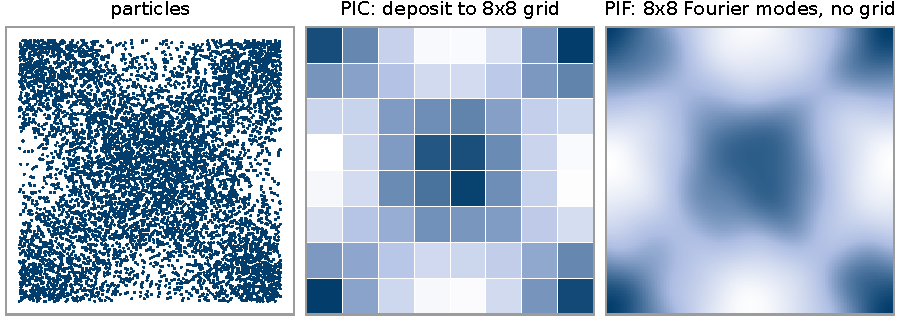
\includegraphics[width=0.55\textwidth]{pic_vs_pif}\\[-2pt]
  {\tiny\color{fzjgray80} Illustration with synthetic particles, both with 64 degrees of freedom}\par
  \vspace{8pt}
  \begin{columns}[T]
    \begin{column}{0.44\textwidth}
      \small\textbf{PIC: the grid causes trouble}\\[4pt]
      \begin{tikzpicture}[mcap/.style={anchor=north, text width=2.5cm, align=center, font=\tiny}]
        % aliasing: k=7/8 sampled on 8 points looks like k=-1/8
        \begin{scope}[x=0.28cm, y=0.32cm]
          \draw[fzjblue!60, thin, domain=0:8, samples=120] plot (\x, {sin(360*0.875*\x)});
          \draw[fzjred, thick, dashed, domain=0:8, samples=60] plot (\x, {-sin(360*0.125*\x)});
          \foreach \i in {0,...,8} \fill (\i, {-sin(360*0.125*\i)}) circle (1.1pt);
          \node[mcap] at (4,-1.4) {\textbf{aliasing} $\to$ grid heating, energy drift};
        \end{scope}
        % Debye length vs cell size
        \begin{scope}[shift={(3.3,0)}]
          \draw[fzjgray50, step=0.32] (0,-0.32) grid (1.6,0.32);
          \draw[fzjred, thick] (0.8,0) circle (0.32);
          \node[mcap] at (0.8,-0.45) {cells must resolve the \textbf{Debye length}};
        \end{scope}
      \end{tikzpicture}
    \end{column}
    \begin{column}{0.54\textwidth}
      \small\textbf{PIF: particles talk to Fourier modes}
      \begin{itemize}\scriptsize
        \item $\hat\rho_k = S_k \sum_j q_j\, e^{-i k\cdot x_j}$ - no real-space grid
        \item No grid aliasing, spectral accuracy
        \item With NUFFTs: same cost order as PIC, higher constant
        \item Limits: global operation; periodic / free-space boundaries
      \end{itemize}
    \end{column}
  \end{columns}
  \src{Mitchell et al., J.\ Comput.\ Phys.\ 396 (2019); Barnes \& Chac\'on, arXiv:1910.10833}
\end{frame}

% - frame 3 - GO20: slide 22 (PDF p.23); scaling: slide 18 (PDF p.19)
\begin{frame}{Why learn the field operator?}
  \centering
  \begin{tikzpicture}[tile/.style={sim, minimum width=3.6cm, minimum height=1.35cm}]
    \node[tile] (a) at (0,0)   {{\Large $\sim 10^{11}$}\\[2pt] grid points / modes};
    \node[tile] (b) at (4.1,0) {{\Large $\sim 10^{12}$}\\[2pt] particles};
    \node[tile] (c) at (8.2,0) {{\Large $\sim 10^{5}$}\\[2pt] time steps};
    \node[font=\scriptsize, text=fzjgray80, below=2pt of b] {for one high-fidelity run (fusion, particle accelerators)};
  \end{tikzpicture}
  \vspace{2pt}
  \begin{columns}[t]
    \begin{column}{0.4\textwidth}
      \begin{itemize}\small
        \item PIC and PIF \hl{do} scale well on today's supercomputers
        \item High-fidelity and many-query studies remain \hl{too expensive}
      \end{itemize}
    \end{column}
    \begin{column}{0.56\textwidth}
      {\small\textbf{Hypotheses of the NEOPIC project}}
      \begin{itemize}\scriptsize
        \item Implicit / larger time steps via autograd Jacobians
        \item Differentiable simulations
        \item Field operators that are expensive or not known exactly
        \item One model for many codes
      \end{itemize}
    \end{column}
  \end{columns}
  \vspace{4pt}
  \fcolorbox{fzjblue}{fzjblue!6}{\parbox{0.92\textwidth}{\scriptsize
    By operation count, one inference step costs more than one PIF step: the model applies the
    PIF-type transform $2L$ times per step for $d_v$ channels. Whether that pays off over a whole
    simulation is open; \hl{scaling and coupling} are the prerequisites to find out.}}
  \src{Numbers: Muralikrishnan, Go20 2026}
\end{frame}

% - frame 4 - GO20: none
\begin{frame}{Deep learning surrogates}
  \begin{columns}[c]
    \begin{column}{0.5\textwidth}
      \begin{itemize}\small
        \item \hl{Foundation models}: pretrain once, fine-tune for new tasks
        \item \hl{Function to function}: not tied to one grid or resolution"
        \item Precedent - \textbf{Poseidon} (Herde et al., NeurIPS 2024): pretrained on a \emph{small} set of
          fluid PDEs (compressible Euler, incompressible Navier--Stokes), generalises to unseen PDEs
        \item \hl{Differentiable} end to end: gradients for optimisation, inverse problems, implicit time stepping
      \end{itemize}
    \end{column}
    \begin{column}{0.48\textwidth}
      \centering
      \begin{tikzpicture}
        % grid / image data
        \foreach \i in {0,...,7} \foreach \j in {0,...,7} {
          \pgfmathsetmacro{\v}{50+45*sin(45*\i)*cos(45*\j)}
          \fill[fzjblue!\v] (0.3*\i, 0.3*\j) rectangle ++(0.3,0.3);
        }
        \node[font=\scriptsize, align=center] at (1.2,-0.45) {fields on a grid\\(Poseidon)};
        % particle data
        \pgfmathsetseed{3}
        \begin{scope}[shift={(3.2,0)}]
          \draw[fzjgray50] (0,0) rectangle (2.4,2.4);
          \foreach \i in {1,...,160} {
            \pgfmathsetmacro{\px}{1.2+0.9*rand}
            \pgfmathsetmacro{\py}{1.2+0.9*rand}
            \fill[fzjblue] (\px,\py) circle (0.8pt);
          }
          \node[font=\scriptsize, align=center] at (1.2,-0.45) {particles anywhere\\(our data)};
        \end{scope}
        \draw[arr, fzjred] (2.55,1.2) -- node[above, font=\Large] {?} (3.05,1.2);
      \end{tikzpicture}
    \end{column}
  \end{columns}
  \src{Herde et al., Poseidon, NeurIPS 2024, arXiv:2405.19101}
\end{frame}

% - frame 5 - GO20: slide 23 (PDF p.24)
\begin{frame}{The project's approach}
  \begin{columns}[c]
    \begin{column}{0.44\textwidth}
      \centering
      \begin{tikzpicture}
        \node[ml, minimum width=4.0cm, minimum height=1.35cm] (no) at (0,1.3)
          {\textbf{Neural operator}\\ $x \mapsto E$\\[-1pt]
           {\scriptsize\color{fzjgray80} replaces scatter + solve + gather}};
        \node[sim, minimum width=4.0cm, minimum height=0.9cm] (pu) at (0,-1.3)
          {\textbf{Push} (classical)\\[-1pt]\scriptsize $\dot x=v,\ \dot v=\tfrac{q}{m}E$};
        \draw[arr] (no.east) to[out=-30, in=30] node[right, font=\scriptsize] {$E$} (pu.east);
        \draw[arr] (pu.west) to[out=150, in=210] node[left, font=\scriptsize] {$x$} (no.west);
        \node[simlight, minimum width=1.6cm] (in) at (0,2.65) {\scriptsize Init $x, v, q$};
        \draw[arr, fzjblue] (in) -- (no);
      \end{tikzpicture}
    \end{column}
    \begin{column}{0.54\textwidth}
      \begin{itemize}\small
        \item Learn the whole map $P^{T} \mathcal{L}^{-1} P : x \mapsto E$\\
          {\scriptsize electrostatic: $E$ depends on the positions only}
        \item Particle push stays classical
        \item Training data from mini-apps (PIF/PIC)
        \item Input: particle positions $\to$ output: $E$ at the particles
      \end{itemize}
    \end{column}
  \end{columns}
\end{frame}

% - frame 6 - GO20: slide 24 (PDF p.25)
\begin{frame}{The model: nonuniform FNO}
  \centering
  \begin{tikzpicture}[node distance=0.9cm]
    \node[simlight, minimum height=1cm] (x) {$x_p$\\[-1pt]\scriptsize $d\times N$};
    \node[ml, right=of x, minimum height=1cm] (P) {lift $P$};
    \node[ml, right=of P, minimum height=1cm, minimum width=2.6cm] (B) {\textbf{Fourier block}\\[-1pt]\scriptsize $\times L$};
    \node[ml, right=of B, minimum height=1cm] (Q) {project $Q$};
    \node[simlight, right=of Q, minimum height=1cm] (E) {$E(x_p)$\\[-1pt]\scriptsize $d\times N$};
    \draw[arr] (x) -- (P); \draw[arr] (P) -- node[above, font=\tiny] {$d_v\!\times\! N$} (B);
    \draw[arr] (B) -- (Q); \draw[arr] (Q) -- (E);

    % zoom into one Fourier block
    \begin{scope}[shift={(-0.2,-3.0)}, node distance=0.55cm]
      \node[box, draw=fzjgray50, minimum height=0.9cm] (v) at (0,0) {$v$\\[-1pt]\tiny $d_v\times N$};
      \node[mllight, right=of v, minimum height=0.9cm] (F) {NUFFT / NUDFT\\[-1pt]\tiny $\hat v_k=\sum_p v_p e^{-ik\cdot x_p}$};
      \node[mllight, right=0.8cm of F, minimum height=0.9cm] (R) {$R_k\,\hat v_k$\\[-1pt]\tiny learned, $m$ modes};
      \node[mllight, right=of R, minimum height=0.9cm] (Fi) {inverse NUFFT / NUDFT\\[-1pt]\tiny at the particles $x_p$};
      \node[circle, draw, right=of Fi, inner sep=1pt] (plus) {$+$};
      \node[box, right=0.4cm of plus] (sig) {$\sigma$};
      \node[mllight, below=0.35cm of R] (W) {$W v$ \tiny(pointwise)};
      \draw[arr] (v) -- (F); \draw[arr] (F) -- node[below, font=\tiny] {$m\!\times\! d_v$} (R);
      \draw[arr] (R) -- (Fi); \draw[arr] (Fi) -- (plus); \draw[arr] (plus) -- (sig);
      \draw[arr] (v) |- (W); \draw[arr] (W) -| (plus);
      \draw[brace, fzjblue] ([yshift=3pt]F.north west) -- ([yshift=3pt]Fi.north east)
        node[midway, above=5pt, font=\scriptsize, text=fzjblue, fill=white, inner sep=1pt]
        {a learnable PIF step in latent space};
      \node[draw=fzjgray50, dashed, rounded corners, fit=(v)(sig)(W)(F), inner sep=4pt,
        yshift=0.25cm, minimum height=2.6cm] (zoom) {};
    \end{scope}
    \begin{scope}[on background layer]
      \draw[fzjgray50, dashed] (B.south west) -- (zoom.north west);
      \draw[fzjgray50, dashed] (B.south east) -- (zoom.north east);
    \end{scope}
  \end{tikzpicture}

\end{frame}

% - frame 7 - what goes in, what comes out (grid moved here from "The project")
\begin{frame}{What goes in, what comes out}
  \centering
  \begin{tikzpicture}[
      cell/.style={draw=fzjgray50, fill=fzjgray, rounded corners=2pt, minimum size=0.8cm, inner sep=0pt},
      cloud/.style={draw=fzjgray50, fill=fzjgray, rounded corners=2pt, minimum size=1.3cm, inner sep=0pt},
      head/.style={font=\small\bfseries, text=fzjblue, anchor=north},
      lbl/.style={font=\scriptsize, align=center, anchor=north},
      ar/.style={{Stealth}-{Stealth}, fzjorange!90!black, very thick}]

    % ---- (1) one sample: x -> model -> E -------------------------------------
    \node[head] at (1.2,0.75) {One sample};
    \node[cloud] (xin) at (1.2,-1.0) {};
    \pgfmathsetseed{5}
    \foreach \i in {1,...,30}
      \fill[fzjblue] ($(xin)+(0.55*rand, 0.55*rand)$) circle (0.9pt);
    \node[font=\scriptsize, anchor=west] at (xin.east) {$x$: $3\times N$};
    \node[ml, minimum width=1.6cm, minimum height=0.6cm] (mod) at (1.2,-2.35) {\textbf{NUFNO}};
    \node[cloud] (eout) at (1.2,-3.7) {};
    \pgfmathsetseed{5}   % same particles as above
    \foreach \i in {1,...,30} {
      \pgfmathsetmacro{\px}{0.55*rand}
      \pgfmathsetmacro{\py}{0.55*rand}
      \fill[fzjblue] ($(eout)+(\px,\py)$) circle (0.9pt);
      \draw[-{Stealth[length=1mm]}, fzjorange!90!black, semithick]
        ($(eout)+(\px,\py)$) -- ++({0.15*sin(300*\px)}, 0);
    }
    \node[font=\scriptsize, anchor=west] at (eout.east) {$E$: $3\times N$};
    \draw[arr] (xin) -- (mod);
    \draw[arr] (mod) -- (eout);
    \node[lbl] at (1.2,-4.45) {input: particle positions\\output: $E$ at each particle};

    \draw[fzjgray50] (3.35,0.7) -- (3.35,-5.0);

    % ---- (2) training: d_p rows x t_p columns, each cell one GPU --------------
    \node[head] at (6.0,0.75) {Training};
    \pgfmathsetseed{11}
    \foreach \r/\col in {0/fzjblue, 1/fzjviolet} {
      \foreach \c in {0,...,3} {
        % shadows: each GPU holds a stack of b samples
        \node[cell, fill=fzjgray!70] at ($(4.5+0.95*\c, -1.0-1.45*\r)+(0.1,0.1)$) {};
        \node[cell, fill=fzjgray!85] at ($(4.5+0.95*\c, -1.0-1.45*\r)+(0.05,0.05)$) {};
        \node[cell] (g\r\c) at (4.5+0.95*\c, -1.0-1.45*\r) {};
        \foreach \i in {1,...,10}
          \fill[\col] ($(g\r\c)+(0.3*rand, 0.3*rand)$) circle (0.8pt);
      }
      \draw[ar] ([yshift=-0.55cm]g\r0.center) -- ([yshift=-0.55cm]g\r3.center);
      \node[font=\tiny, fill=white, inner sep=1pt, text=fzjorange!70!black]
        at ($(g\r1)!0.5!(g\r2)+(0,-0.55)$) {all\_reduce: Fourier modes};
    }
    \draw[brace] ([yshift=5pt]g00.north west) -- ([yshift=5pt]g03.north east)
      node[midway, above=3pt, font=\tiny] {$t_p$ particle shards};
    \node[font=\tiny, anchor=east, align=right] at ($(g00.west)!0.5!(g10.west)+(-0.05,0)$) {$d_p$\\sample\\groups};
    % gradient sync between the rows (data parallel), training only
    \draw[ar, dashed] ([xshift=0.3cm]g03.east) -- ([xshift=0.3cm]g13.east)
      node[midway, right=1pt, font=\tiny, align=left, text=fzjorange!70!black] {gradient\\all\_reduce\\(training\\only)};
    \node[lbl] at (6.0,-3.55) {each cell = one GPU, holding\\$b$ samples $\times$ $n$ particles};
    \node[lbl, font=\small] at (6.0,-4.4) {$W = d_p\, t_p$ \quad $b = B/d_p$ \quad $n = N/t_p$};

    \draw[fzjgray50] (9.15,0.7) -- (9.15,-5.0);

    % ---- (3) inference: one row ----------------------------------------------
    \node[head] at (11.4,0.75) {Inference};
    \pgfmathsetseed{11}
    \foreach \c in {0,...,3} {
      \node[cell] (h\c) at (10.0+0.95*\c, -1.0) {};
      \foreach \i in {1,...,10}
        \fill[fzjblue] ($(h\c)+(0.3*rand, 0.3*rand)$) circle (0.8pt);
    }
    \draw[ar] ([yshift=-0.55cm]h0.center) -- ([yshift=-0.55cm]h3.center);
    \node[font=\tiny, fill=white, inner sep=1pt, text=fzjorange!70!black]
      at ($(h1)!0.5!(h2)+(0,-0.55)$) {all\_reduce: Fourier modes};
    \draw[brace] ([yshift=5pt]h0.north west) -- ([yshift=5pt]h3.north east)
      node[midway, above=3pt, font=\tiny] {$t_p$ particle shards};
    \node[lbl] at (11.4,-2.2) {$B = 1$: one configuration\\per time step};
    \node[lbl, font=\small] at (11.4,-3.2) {$d_p = 1$, \quad $W = t_p$};
  \end{tikzpicture}
\end{frame}

% ============================================================
\section{The project and the contribution}    % third 2: how we solve it, frames 7--11
\makesection
% ============================================================

% - frame 7 - GO20: none
\begin{frame}{The project}
  \begin{itemize}\small
    \item NUFNO model
    \item Distributed training: data parallel ($d_p$) $\times$ particle decomposition ($t_p$)
    \item {\scriptsize $t_p$ (\emph{tensor parallel} in the code) = particle decomposition}
    \item \texttt{picND}: evaluation against a PIF reference
    \item Training data from the mini-apps
  \end{itemize}

  \vspace{6pt}
  \visible<2->{
  \centering
  \begin{tikzpicture}[card/.style={simlight, minimum width=4.3cm, minimum height=1.55cm, text width=3.9cm,
      align=flush left, font={\scriptsize\hyphenpenalty 10000 }}]
    \node[card] (a) at (0,0)   {\textbf{\small Scaling inference out}\\[2pt]
      from one GPU holding all particles to many GPUs};
    \node[card] (b) at (4.6,0) {\textbf{\small Leaner I/O}\\[2pt]
      each rank reads only the particles it needs};
    \node[card] (c) at (9.2,0) {\textbf{\small Into IPPL }\\[2pt]
      run the model as a surrogate inside a simulation library};
    \node[anchor=south west, font=\small\bfseries, text=fzjblue] at ([yshift=2pt]a.north west) {The contributions made:};
  \end{tikzpicture}
  }
\end{frame}

% - frame 8 - GO20: none
\begin{frame}{Training I/O: sharded HDF5 reads}
  \begin{columns}[T]
    \begin{column}{0.55\textwidth}
      \centering
      \begin{tikzpicture}
        \foreach \c in {0,...,3} \node[simlight, minimum width=1.2cm, font=\scriptsize] (r\c) at (1.55*\c, -2) {rank \c};
        \only<1>{
          \node[neutral, minimum width=6cm, minimum height=0.55cm] (h5) at (2.32,0) {HDF5 sample: $N$ particles};
          \foreach \c in {0,...,3} \draw[arr, fzjred] (h5.south) -- node[pos=0.75, fill=white, inner sep=1pt, font=\tiny] {$N$} (r\c.north);
          \node[font=\scriptsize, text=fzjred] at (2.32,-2.75) {before: each rank reads $N$, keeps $N/t_p$};
        }
        \only<2->{
          \foreach \c/\col in {0/fzjblue, 1/fzjgreen, 2/fzjviolet, 3/fzjlightblue}
            \node[box, fill=\col, minimum width=1.5cm, minimum height=0.55cm, inner sep=0pt] (s\c) at (1.55*\c,0) {};
          \node[font=\scriptsize] at (2.32,0.5) {HDF5 sample: $N$ particles};
          \foreach \c in {0,...,3} \draw[arr] (s\c.south) -- node[right, font=\tiny] {$N/t_p$} (r\c.north);
          \node[font=\scriptsize, text=fzjblue] at (2.32,-2.75) {after: each rank reads only its shard};
        }
      \end{tikzpicture}
      \vspace{4pt}
      \begin{itemize}\small
        \item<2-> Read volume per rank: $N \to N/t_p$
        \item<3-> Peak GPU memory \hl{unchanged}: set downstream by activations / Fourier layers
      \end{itemize}
    \end{column}
    \begin{column}{0.43\textwidth}
      \visible<3->{
      \centering
      {\small\textbf{Why a larger $t_p$ did not lower peak memory}}\\
      {\scriptsize ($W = 8$ GPUs fixed)}\\[4pt]
      \begin{tikzpicture}[x=1cm, y=1cm]
        % both shards drawn from the origin: same area b*n
        \fill[fzjblue, opacity=0.75] (0,0) rectangle (3.6,0.45);
        \fill[fzjviolet, opacity=0.75] (0,0) rectangle (0.45,1.8);
        \node[font=\scriptsize, anchor=west, text=fzjblue] at (1.2,0.7) {$t_p=2$: \textbf{22222\,MiB}};
        \node[font=\scriptsize, anchor=west, text=fzjviolet!80!black] at (0.6,1.5) {$t_p=8$: \textbf{22222\,MiB}};
        \draw[->] (0,0) -- (4.0,0) node[below left, font=\tiny] {shard size $n = N/t_p$};
        \draw[->] (0,0) -- (0,2.1) node[above right, font=\tiny] {local batch $b = B\,t_p/W$};
      \end{tikzpicture}\\[4pt]
      \fcolorbox{fzjblue}{fzjblue!8}{\small $b\cdot n = \dfrac{B\,N}{W}$ \ independent of $t_p$}
      }
    \end{column}
  \end{columns}
\end{frame}

% - frame 9 - GO20: none
\begin{frame}{Parallel inference}
  \centering
  \sbox{\diagbox}{%
  \begin{tikzpicture}[node distance=0.4cm, every node/.style={font=\scriptsize}]
    \foreach \r/\y in {0/0, 1/-1.05, 2/-2.1} {
      \node[simlight, minimum width=2.2cm, minimum height=0.75cm] (p\r) at (0,\y) {particles of rank \r};
      \node[mllight, minimum width=2.4cm, minimum height=0.75cm, right=of p\r] (m\r) {partial modes $\hat v^{(\r)}_k$};
    }
    \node[ml, minimum height=2.85cm, minimum width=1.5cm, right=0.6cm of m1] (ar)
      {\textbf{all\_reduce}\\[2pt]$\sum_r \hat v^{(r)}_k$};
    \foreach \r in {0,1,2} {
      \draw[arr] (p\r) -- (m\r);
      \draw[arr] (m\r.east) -- (m\r.east -| ar.west);
      \node[mllight, minimum width=2.2cm, minimum height=0.75cm, anchor=west] (f\r) at ($(m\r.east -| ar.east)+(0.6,0)$) {all modes $\hat v_k$};
      \node[simlight, minimum width=2.2cm, minimum height=0.75cm, right=of f\r] (e\r) {$E$ at own particles};
      \draw[arr] (f\r.west -| ar.east) -- (f\r);
      \draw[arr] (f\r) -- (e\r);
    }
    \node[below=2pt of ar, align=center, text=fzjorange!60!black] {payload $O(d_v\, m)$\\ \textbf{independent of $N$}};
    \node[above=2pt of m0, text=fzjgray80] {$\hat v^{(r)}_k=\sum_{p\in r} v_p\, e^{-ik\cdot x_p}$};
  \end{tikzpicture}}%
  % correctness plot (field energy vs time, several GPU counts) appears once the file exists
  \iffig{inference_energy_gpus}{%
    \begin{columns}[c]
      \begin{column}{0.6\textwidth}\centering\resizebox{\linewidth}{!}{\usebox{\diagbox}}\end{column}
      \begin{column}{0.38\textwidth}\centering
        \includegraphics[width=\linewidth, height=4.2cm, keepaspectratio]{inference_energy_gpus}\\
        {\scriptsize field energy vs.\ time, several GPU counts}
      \end{column}
    \end{columns}}{\usebox{\diagbox}}

  \vspace{6pt}
  \begin{itemize}\small
    \item Particle decomposition in \texttt{picND}: each GPU holds $N/W$ particles;
      in inference $W = t_p$ (no data parallelism)
    \item Integrated quantities (e.g.\ field energy) also via all\_reduce
  \end{itemize}
\end{frame}

% - frame 10 - rank layout; correctness plot on <2> once the file exists
\begin{frame}{Coupling to IPPL}
  \begin{columns}[c]
    \begin{column}{0.52\textwidth}
      \centering
      \only<1>{%
  \begin{tikzpicture}[scale=0.72, every node/.append style={transform shape}]
    \foreach \r in {0,1,2} {
      \node[sim, minimum width=2.6cm, minimum height=0.85cm] (ip\r) at (3.6*\r, 0) {\textbf{IPPL} (C++)\\[-1pt]\scriptsize Kokkos::View on GPU};
      \node[ml,  minimum width=2.6cm, minimum height=0.85cm] (pt\r) at (3.6*\r, -1.9) {\textbf{PyTorch}\\[-1pt]\scriptsize embedded Python};
      \draw[{Stealth}-{Stealth}, very thick] (ip\r) -- node[right, font=\tiny, align=left] {DLPack\\zero-copy} (pt\r);
      \node[draw=fzjgray50, rounded corners, fit=(ip\r)(pt\r), inner sep=5pt,
        label={[font=\scriptsize, text=fzjgray80]above:MPI rank \r\ = GPU \r}] (rk\r) {};
    }
    \foreach \a/\b in {0/1, 1/2} {
      \draw[fzjblue, thick, {Stealth}-{Stealth}] (ip\a.east) -- (ip\b.west);
      \draw[fzjorange!90!black, thick, {Stealth}-{Stealth}] (pt\a.east) -- (pt\b.west);
    }
    % legend for the inter-rank arrows
    \draw[fzjblue, thick, {Stealth}-{Stealth}] ($(rk0.south west)+(0,-0.35)$) -- ++(0.8,0)
      node[right, font=\scriptsize, text=fzjblue] {MPI inside IPPL};
    \draw[fzjorange!90!black, thick, {Stealth}-{Stealth}] ($(rk1.south west)+(0,-0.35)$) -- ++(0.8,0)
      node[right, font=\scriptsize, text=fzjorange!60!black] {all\_reduce inside the model};
  \end{tikzpicture}}%
      \only<1>{\\[10pt]%
      \begin{tikzpicture}[layer/.style={sim, minimum width=5.2cm, minimum height=0.45cm, font=\tiny, inner sep=1pt}]
        \node[simlight, minimum width=5.2cm, minimum height=0.45cm, font=\tiny, inner sep=1pt] (app) {mini-app, e.g.\ Landau damping};
        \node[layer, below=1.5pt of app] (ip) {IPPL: particles, fields, solvers};
        \node[layer, below=1.5pt of ip, minimum width=2.55cm, xshift=-1.325cm] {Kokkos};
        \node[layer, below=1.5pt of ip, minimum width=2.55cm, xshift=1.325cm] {MPI};
        \node[neutral, below=0.5cm of ip, minimum width=5.2cm, minimum height=0.4cm, font=\tiny, inner sep=1pt] {CPU \;$\cdot$\; GPU};
      \end{tikzpicture}
      }%
      \iffig{ippl_model_vs_pif}{\only<2>{%
        \includegraphics[width=\linewidth, height=5cm, keepaspectratio]{ippl_model_vs_pif}\\
        {\scriptsize IPPL + model vs.\ IPPL's own PIF solver}}}{}
    \end{column}
    \begin{column}{0.46\textwidth}
      \begin{itemize}\small
        \item IPPL: C++ particle--mesh library, performance portable (Kokkos + MPI);
          underlies the production accelerator code OPAL-X
        \item Time step unchanged: only the \hl{field evaluation} is swapped for the model
        \item Opt-in, header-only (pybind11 + DLPack), \hl{no changes to IPPL}
        \item Same MPI rank hosts IPPL and the model: \hl{rank $i$ talks to rank $i$}
        \item Data stays on the GPU; Python writes $E$ \hl{directly into IPPL's memory}
      \end{itemize}
    \end{column}
  \end{columns}
  \src{Muralikrishnan et al., arXiv:2205.11052; Mayani et al., PASC '26, arXiv:2605.05469}
\end{frame}

% - frame 11 - REAL results only: figures from the IPPL-interop deck (p.13, p.14)
\begin{frame}{Scaling results}
  \centering
  {\small NUFFT model, run \hl{through the IPPL interop layer}: 400 time steps, 1--512 GPUs, up to 1.6\,B particles}\\[6pt]
  \figorph{ippl_inference_scaling}{6.9cm}{4.6cm}{Strong + weak scaling}{IPPL-interop deck p.13}
  \hfill
  \figorph{ippl_scaling_efficiency}{6.9cm}{4.6cm}{Scaling efficiency}{IPPL-interop deck p.14}\\[4pt]
  {\scriptsize\color{fzjgray80} efficiency: strong $E_s = P_0\,T(P_0)\,/\,(P\,T(P))$, \quad weak $E_w = T_\mathrm{base}/T(P)$}
\end{frame}

% ============================================================
\section{Deep dive}      % third 3: look at this crazy thing, frames 12--15
\makesection
% ============================================================

% - frame 12 - GO20: slides 16--17 (PDF p.17--18)
\begin{frame}{Two ways to split the particles}
  \centering
  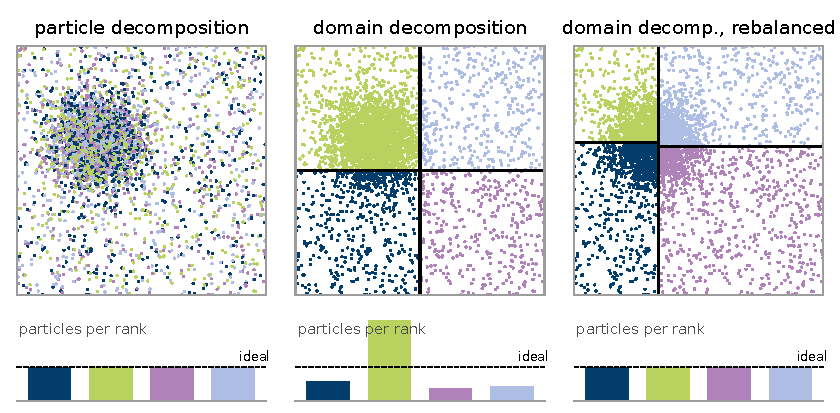
\includegraphics[width=0.54\textwidth]{decomposition_balance}\\[-2pt]
  {\tiny\color{fzjgray80} Illustration with synthetic particles (beam on a background), 4 ranks}
  \vspace{2pt}
  \begin{columns}[t]
    \begin{column}{0.48\textwidth}
      \small\textbf{Particle decomposition} (The project's model, \texttt{picND})\\
      {\scriptsize each rank: random subset over the \hl{whole} domain; always balanced; Fourier modes duplicated}
    \end{column}
    \begin{column}{0.48\textwidth}
      \small\textbf{Domain decomposition} (IPPL)\\
      {\scriptsize each rank: \hl{one subdomain}; balance needs re-partitioning $\to$ subdomain boundaries move}
    \end{column}
  \end{columns}
  \vspace{8pt}
  {\scriptsize Under domain decomposition, clustered distributions also unbalance the \hl{model's} work per rank.}
\end{frame}

% - frame 13 - GO20: none (follows from frame 12)
\begin{frame}[fragile]{The bug: local vs.\ global bounds}
  \begin{columns}[c]
    \begin{column}{0.4\textwidth}
      \begin{tikzpicture}
        \node[box, draw=fzjgray50, fill=fzjgray!60, align=left, font=\scriptsize\ttfamily, text width=5.0cm] {%
          {\color{fzjgray80}\# valid(): global bounds}\\
          lo = all\_reduce(x.min(), MIN)\\
          hi = all\_reduce(x.max(), MAX)\\[4pt]
          {\color{fzjred}\# \_\_call\_\_(): local bounds}\\
          {\color{fzjred}lo, hi = x.min(), x.max()}};
      \end{tikzpicture}\\
      {\tiny\color{fzjgray80} schematic, not the actual code}
      \begin{itemize}\scriptsize
        \item Particle decomp.: local $\approx$ global bounds $\to$ \hl{harmless}, invisible in \texttt{picND}
        \item Domain decomp.: each rank stretches its subdomain to $[0,2\pi)$ $\to$ ranks sum modes in
          {\color{fzjred}incompatible coordinates}
        \item \textbf{Fix:} pass global bounds (one all\_reduce, or the known domain size)
      \end{itemize}
    \end{column}
    \begin{column}{0.58\textwidth}
      \centering
      \only<1>{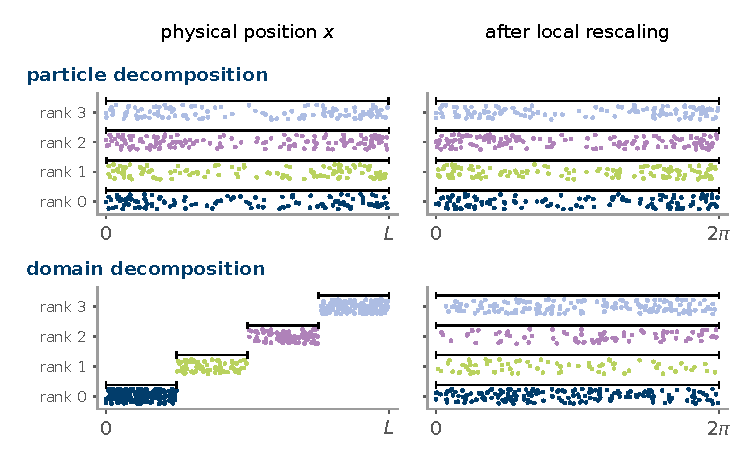
\includegraphics[width=0.8\textwidth]{bug_rescale}}%
      \only<2>{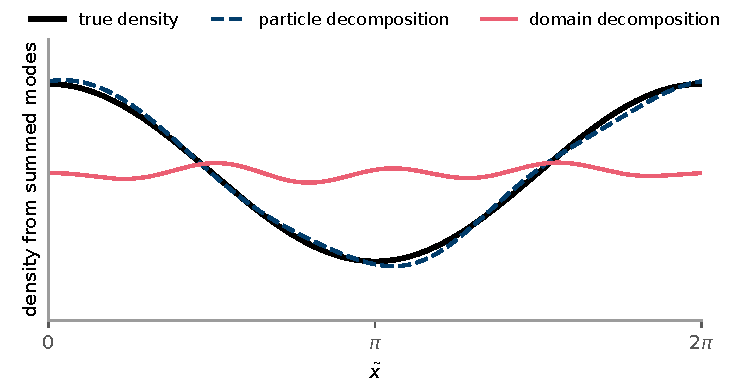
\includegraphics[width=0.8\textwidth]{bug_reconstruct}\\[2pt]
        {\scriptsize Density rebuilt from the all-reduced modes}}\\[2pt]
      {\tiny\color{fzjgray80} Illustration: synthetic 1D density $1+0.6\cos x$, 4 ranks, $|k|\le 4$}
      \visible<2>{\\[4pt]\fcolorbox{fzjblue}{fzjblue!6}{\parbox{0.92\linewidth}{\centering\scriptsize
        The Fourier sum does not care which rank holds which particle: with consistent coordinates
        the model works under \hl{any} decomposition, including IPPL's.}}}
    \end{column}
  \end{columns}
\end{frame}

% - frame 14 - the rising noise floor: same RNG seed on every inference rank
\begin{frame}[fragile]{The rising noise floor}
  \begin{columns}[c]
    \begin{column}{0.4\textwidth}
      \begin{tikzpicture}
        \node[box, draw=fzjgray50, fill=fzjgray!60, align=left, font=\scriptsize\ttfamily, text width=5.0cm] {%
          {\color{fzjred}\# before: same seed on every rank}\\
          {\color{fzjred}cp.random.seed(152)}\\[4pt]
          {\color{fzjgreen!50!black}\# fix: one seed per rank}\\
          {\color{fzjgreen!50!black}cp.random.seed(152 + 100*rank)}};
      \end{tikzpicture}
      \begin{itemize}\scriptsize
        \item Every GPU draws its $N/W$ particles from the \hl{same seed}
          $\to$ very similar particles on all ranks
        \item Effectively only $\approx N/W$ independent particles
          $\to$ noise floor \hl{grows with the GPU count}
        \item One seed per rank $\to$ the noise floor no longer depends on $W$
      \end{itemize}
    \end{column}
    \begin{column}{0.58\textwidth}
      \centering
      \only<1>{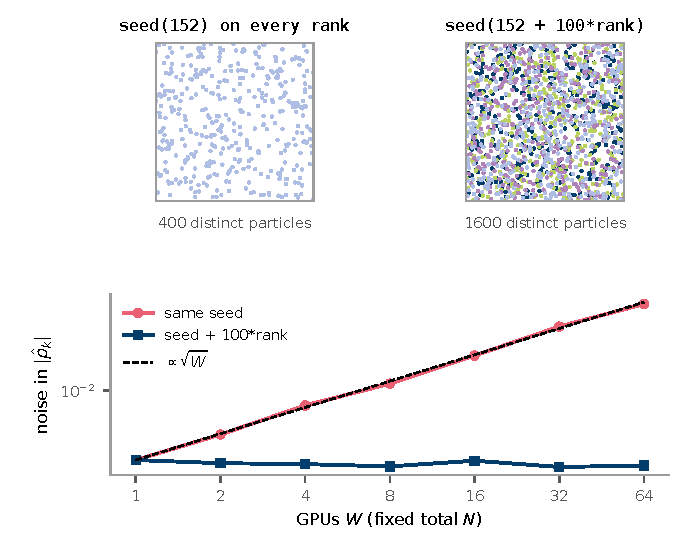
\includegraphics[height=5.5cm]{seed_noise}\\[2pt]
        {\tiny\color{fzjgray80} Illustration: numpy, uniform particles, fixed $N=2^{16}$, modes $k=1..8$, 20 trials}}%
      \iffig{noise_floor_before_after}{\only<2>{%
        \includegraphics[width=8.6cm, height=5.2cm, keepaspectratio]{noise_floor_before_after}}}{}
    \end{column}
  \end{columns}
\end{frame}

% - frame 15 -
\begin{frame}{Zero-copy via DLPack}
  \centering
  \only<1-3>{%
  \begin{tikzpicture}[node distance=0.4cm, every node/.style={font=\scriptsize}]
    % peel the types
    \node[simlight, font=\tiny] (t1) {\texttt{ParticleAttrib<Vector<double,3>>}};
    \node[simlight, font=\tiny, right=of t1] (t2) {\texttt{Kokkos::View<Vector<double,3>*>}};
    \node[simlight, font=\tiny, right=of t2] (t3) {shape $(N,3)$ of \texttt{double}};
    \draw[arr] (t1) -- (t2); \draw[arr] (t2) -- (t3);
    % memory strip
    \begin{scope}[shift={(0.2,-1.55)}]
      \foreach \i/\l in {0/x_0, 1/y_0, 2/z_0, 3/x_1, 4/y_1, 5/z_1, 6/x_2, 7/y_2, 8/z_2}
        \node[draw=fzjblue, fill=fzjblue!12, minimum width=0.75cm, minimum height=0.55cm, inner sep=0pt] (c\i) at (0.75*\i,0) {$\l$};
      \node[right=0pt of c8] (dots) {$\cdots$};
      \node[anchor=west, text=fzjgray80] at ($(dots.east)+(0.1,0)$) {one GPU allocation, no copy};
    \end{scope}
    \node[sim, left=0.9cm of c0] (view) {Kokkos::View};
    \draw[arr, fzjblue] (view) -- (c0);
    \visible<2->{
      \node[ml, align=left, font=\scriptsize\ttfamily, below=0.7cm of c3, anchor=north] (dl) {%
        DLTensor\{ data, device=CUDA,\\
        \ dtype=float64, shape=(N,3),\\
        \ strides=(3,1) \} + deleter};
      \draw[arr, fzjorange!80!black] (dl.north) to[out=90, in=-90] (c0.south);
      \node[right=0.4cm of dl, text width=5.2cm, align=left] {
        \textbf{Zero-copy} only if standard layout, no padding:\\
        \texttt{sizeof(Vector<T,D>) == D*sizeof(T)}\\
        otherwise: \hl{repack on the device} (still no host copy)};
    }
  \end{tikzpicture}
  \vspace{4pt}
  \visible<3->{
  \begin{columns}[t]
    \begin{column}{1\textwidth}
      \small\textbf{Lifetime}\\
      {\scriptsize the capsule keeps the Kokkos View alive until PyTorch releases it}
    \end{column}
  \end{columns}
  }
  }%
  \only<4>{%
  {\small\textbf{Why it matters beyond this project}}\\[6pt]
  \begin{columns}[c]
    \begin{column}{0.6\textwidth}
      \centering
      \begin{tikzpicture}[every node/.style={font=\scriptsize}]
        \node[circle, fill=fzjgray80, text=white, minimum size=1.7cm, align=center] (hub)
          {\textbf{DLPack}\\C ABI};
        \node[sim, minimum width=2.3cm] (ippl) at (-3.2, 0.7) {IPPL};
        \node[simlight, minimum width=2.3cm, dashed] (kok) at (-3.2,-0.7) {any Kokkos code\\[-1pt]\tiny(design property, not tested)};
        \draw[thick, fzjblue] (ippl) -- (hub);
        \draw[thick, fzjblue, dashed] (kok) -- (hub);
        \foreach \n/\y in {PyTorch/1.5, JAX/0.75, CuPy/0, NumPy/-0.75, mpi4py/-1.5} {
          \ifx\n PyTorch
            \node[ml, minimum width=1.7cm] (\n) at (3.0,\y) {\n};
            \draw[thick, fzjorange!90!black] (\n) -- (hub);
          \else
            \node[mllight, minimum width=1.7cm] (\n) at (3.0,\y) {\n};
            \draw[thick, fzjorange!90!black, dashed] (\n) -- (hub);
          \fi
        }
        \node[text=fzjgray80] at (0,1.5) {CPU \;$\cdot$\; CUDA \;$\cdot$\; ROCm \;$\cdot$\; \ldots};
      \end{tikzpicture}
    \end{column}
    \begin{column}{0.38\textwidth}
      \begin{itemize}\small
        \item Open standard: NumPy, CuPy, PyTorch, TensorFlow, JAX, MXNet, TVM, Paddle, mpi4py
        \item Cross-hardware, plain C ABI $\to$ any language
        \item Our export side is generic over Kokkos Views; model side not tied to PyTorch
      \end{itemize}
      \vspace{4pt}
    \end{column}
  \end{columns}
  \src{dmlc.github.io/dlpack}
  }
\end{frame}

% ============================================================
\section{Status}         % the last 1%, frames 16--17
\makesection
% ============================================================

% - frame 16 -
\begin{frame}{Status and outlook}
  \centering
  \begin{tikzpicture}[
      head/.style={box, minimum width=4.6cm, font=\small\bfseries},
      body/.style={box, minimum width=4.6cm, anchor=north, font=\scriptsize}]
    \foreach \x/\t/\c in {0/Works/fzjgreen, 4.85/In progress/fzjyellow, 9.7/Next/fzjlightblue}
      \node[head, fill=\c] (h\x) at (\x,0) {\t};
    \node[body, fill=fzjgreen!15] at (0,-0.4) {%
      \parbox[t][3.2cm][t]{4.3cm}{\raggedright
      \textbullet\ Sharded HDF5 reads in training\\[2pt]
      \textbullet\ Sharded inference in \texttt{picND}\\[2pt]
      \textbullet\ One RNG seed per rank\\[2pt]
      \textbullet\ Global-bounds fix\\[2pt]
      \textbullet\ IPPL $\leftrightarrow$ PyTorch coupling, end to end\\[2pt]
      \textbullet\ Inference scaling through IPPL: up to 512 GPUs, 1.6\,B particles}};
    \node[body, fill=fzjyellow!20] at (4.85,-0.4) {%
      \parbox[t][3.2cm][t]{4.3cm}{\raggedright
      \textbullet\ ADIOS2 / openPMD streaming}};
    \node[body, fill=fzjlightblue!25] at (9.7,-0.4) {%
      \parbox[t][3.2cm][t]{4.3cm}{\raggedright
      \textbullet\ Per-step cost comparison vs.\ IPPL's PIF at scale\\[2pt]
      \textbullet\ Mixed precision\\[2pt]
      \textbullet\ Load balancing for clustered distributions\\[2pt]
      \textbullet\ Testing the time-step hypothesis}};
  \end{tikzpicture}\\[8pt]
  \fcolorbox{fzjblue}{fzjblue!6}{\parbox{0.92\textwidth}{\centering\small
    \textbf{Open question:} does the learned operator pay off over a full simulation compared to PIF?}}
\end{frame}

% - frame 17 -
\begin{frame}{Acknowledgements}
  \begin{columns}[c]
    \begin{column}{0.55\textwidth}
      \begin{itemize}
        \item \textbf{Dr.\ Sriramkrishnan Muralikrishnan} (JSC) -- supervisor
        \item \textbf{Chelsea John} -- the foundation model is her PhD thesis;
          my work contributes to it
        \item NEOPIC is funded by \textbf{Helmholtz AI}\\
          {\scriptsize INF funding code ZT-I-PF-5-242}
      \end{itemize}
    \end{column}
    \begin{column}{0.42\textwidth}
      \centering
      {\huge\color{fzjblue}\textbf{Thank you!}}\\[8pt]
      {\large Questions?}
    \end{column}
  \end{columns}
\end{frame}

\end{document}
